\autsection{Autonomous Landing Site Selection}{Kristian Sloth Lauszus}
%\autsubsection{Image Recognition}{Kristian Sloth Lauszus}
Since the bandwidth from the orbiter to the earth is limited it is beneficial to have a semi-autonomous system that can pick an potential landing site from some given parameters. For instance it would be useful to pick a landing site that does not have any ridges, as there is risk of the lander tipping over after the landing. This could be done by simple edge detection, such as a Laplacian Gaussian filter from a greyscale image. If the system finds a potential landing site the image could then be streamed back to earth either as a binary, greyscale or even the full color image for further analysis. Furthermore object detection could be used to locate certain characteristics. The image could then be cropped and streamed back to earth, thus decreasing the needed bandwidth.

Figure \ref{fig:edge_detection} shows two examples of how a Laplacian Gaussian filter has been used for edge detection on images from the moon. It shows clearly how cracks on the surface show up. These locations could then be picked as potential landing sites and further analysed by the ground control.

\begin{figure}[htb]
	\centering
	\subfloat{
		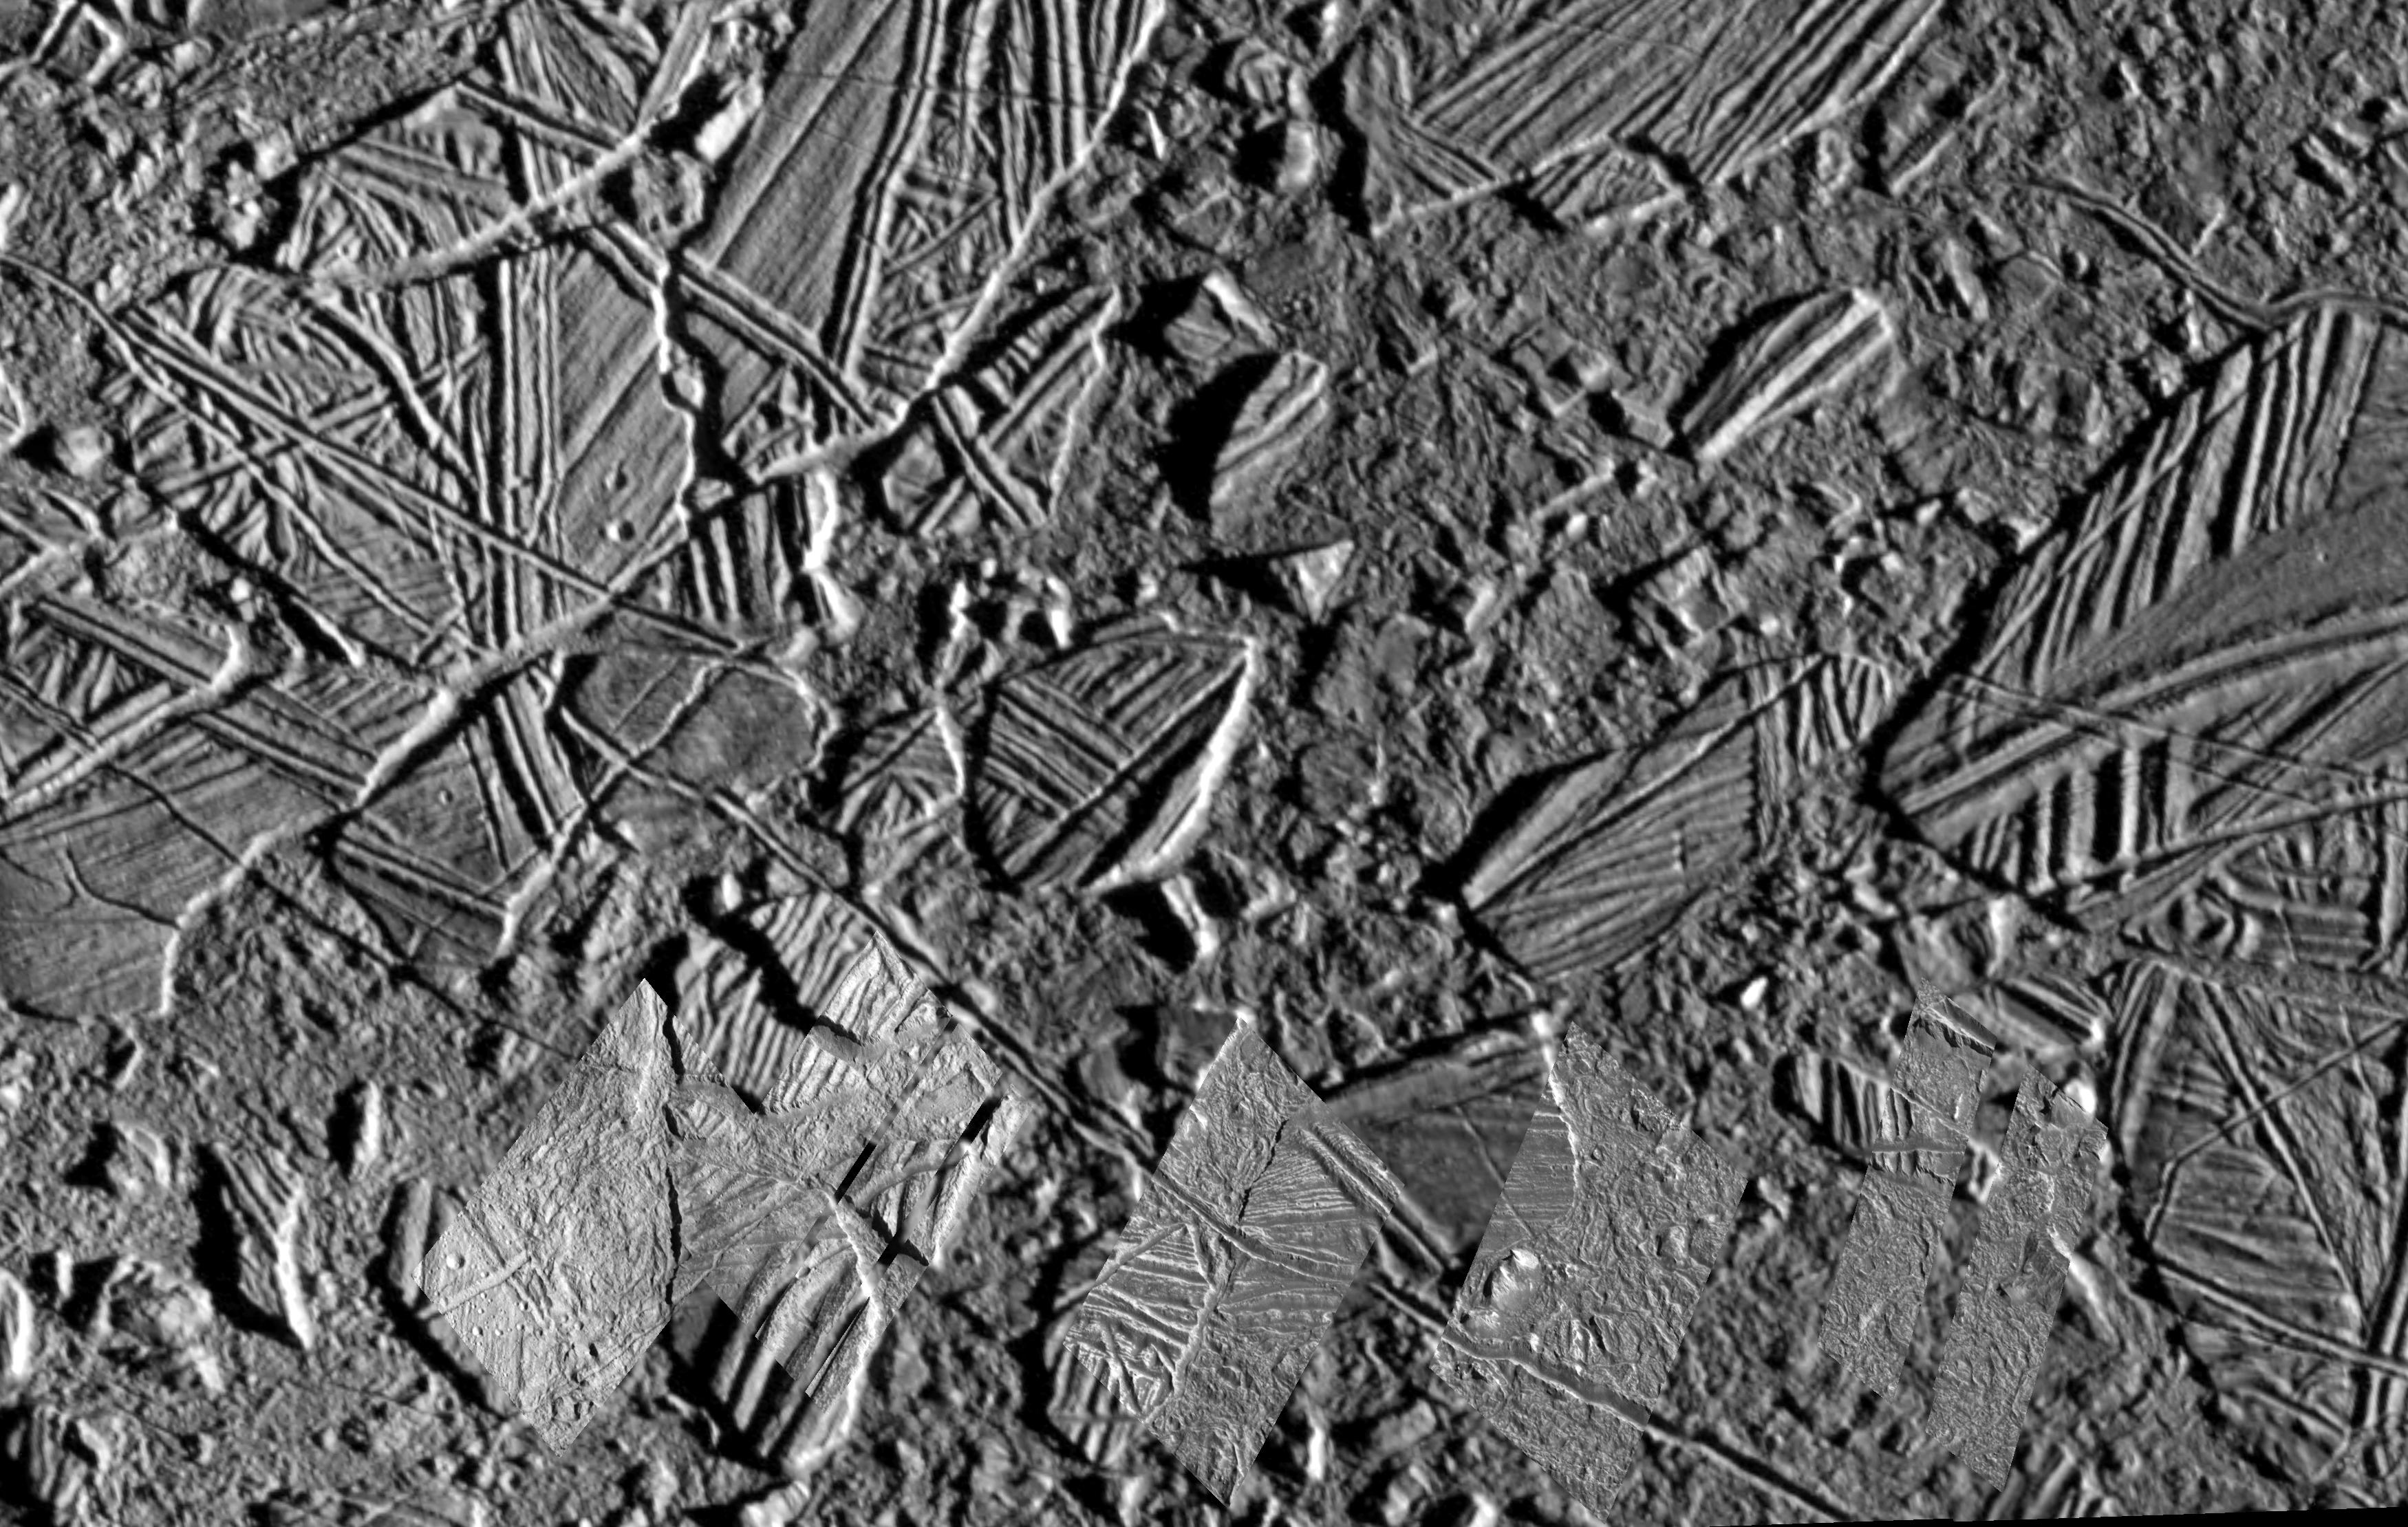
\includegraphics[width=.48\textwidth]{figures/edge/PIA01403}
	}
	\subfloat{
		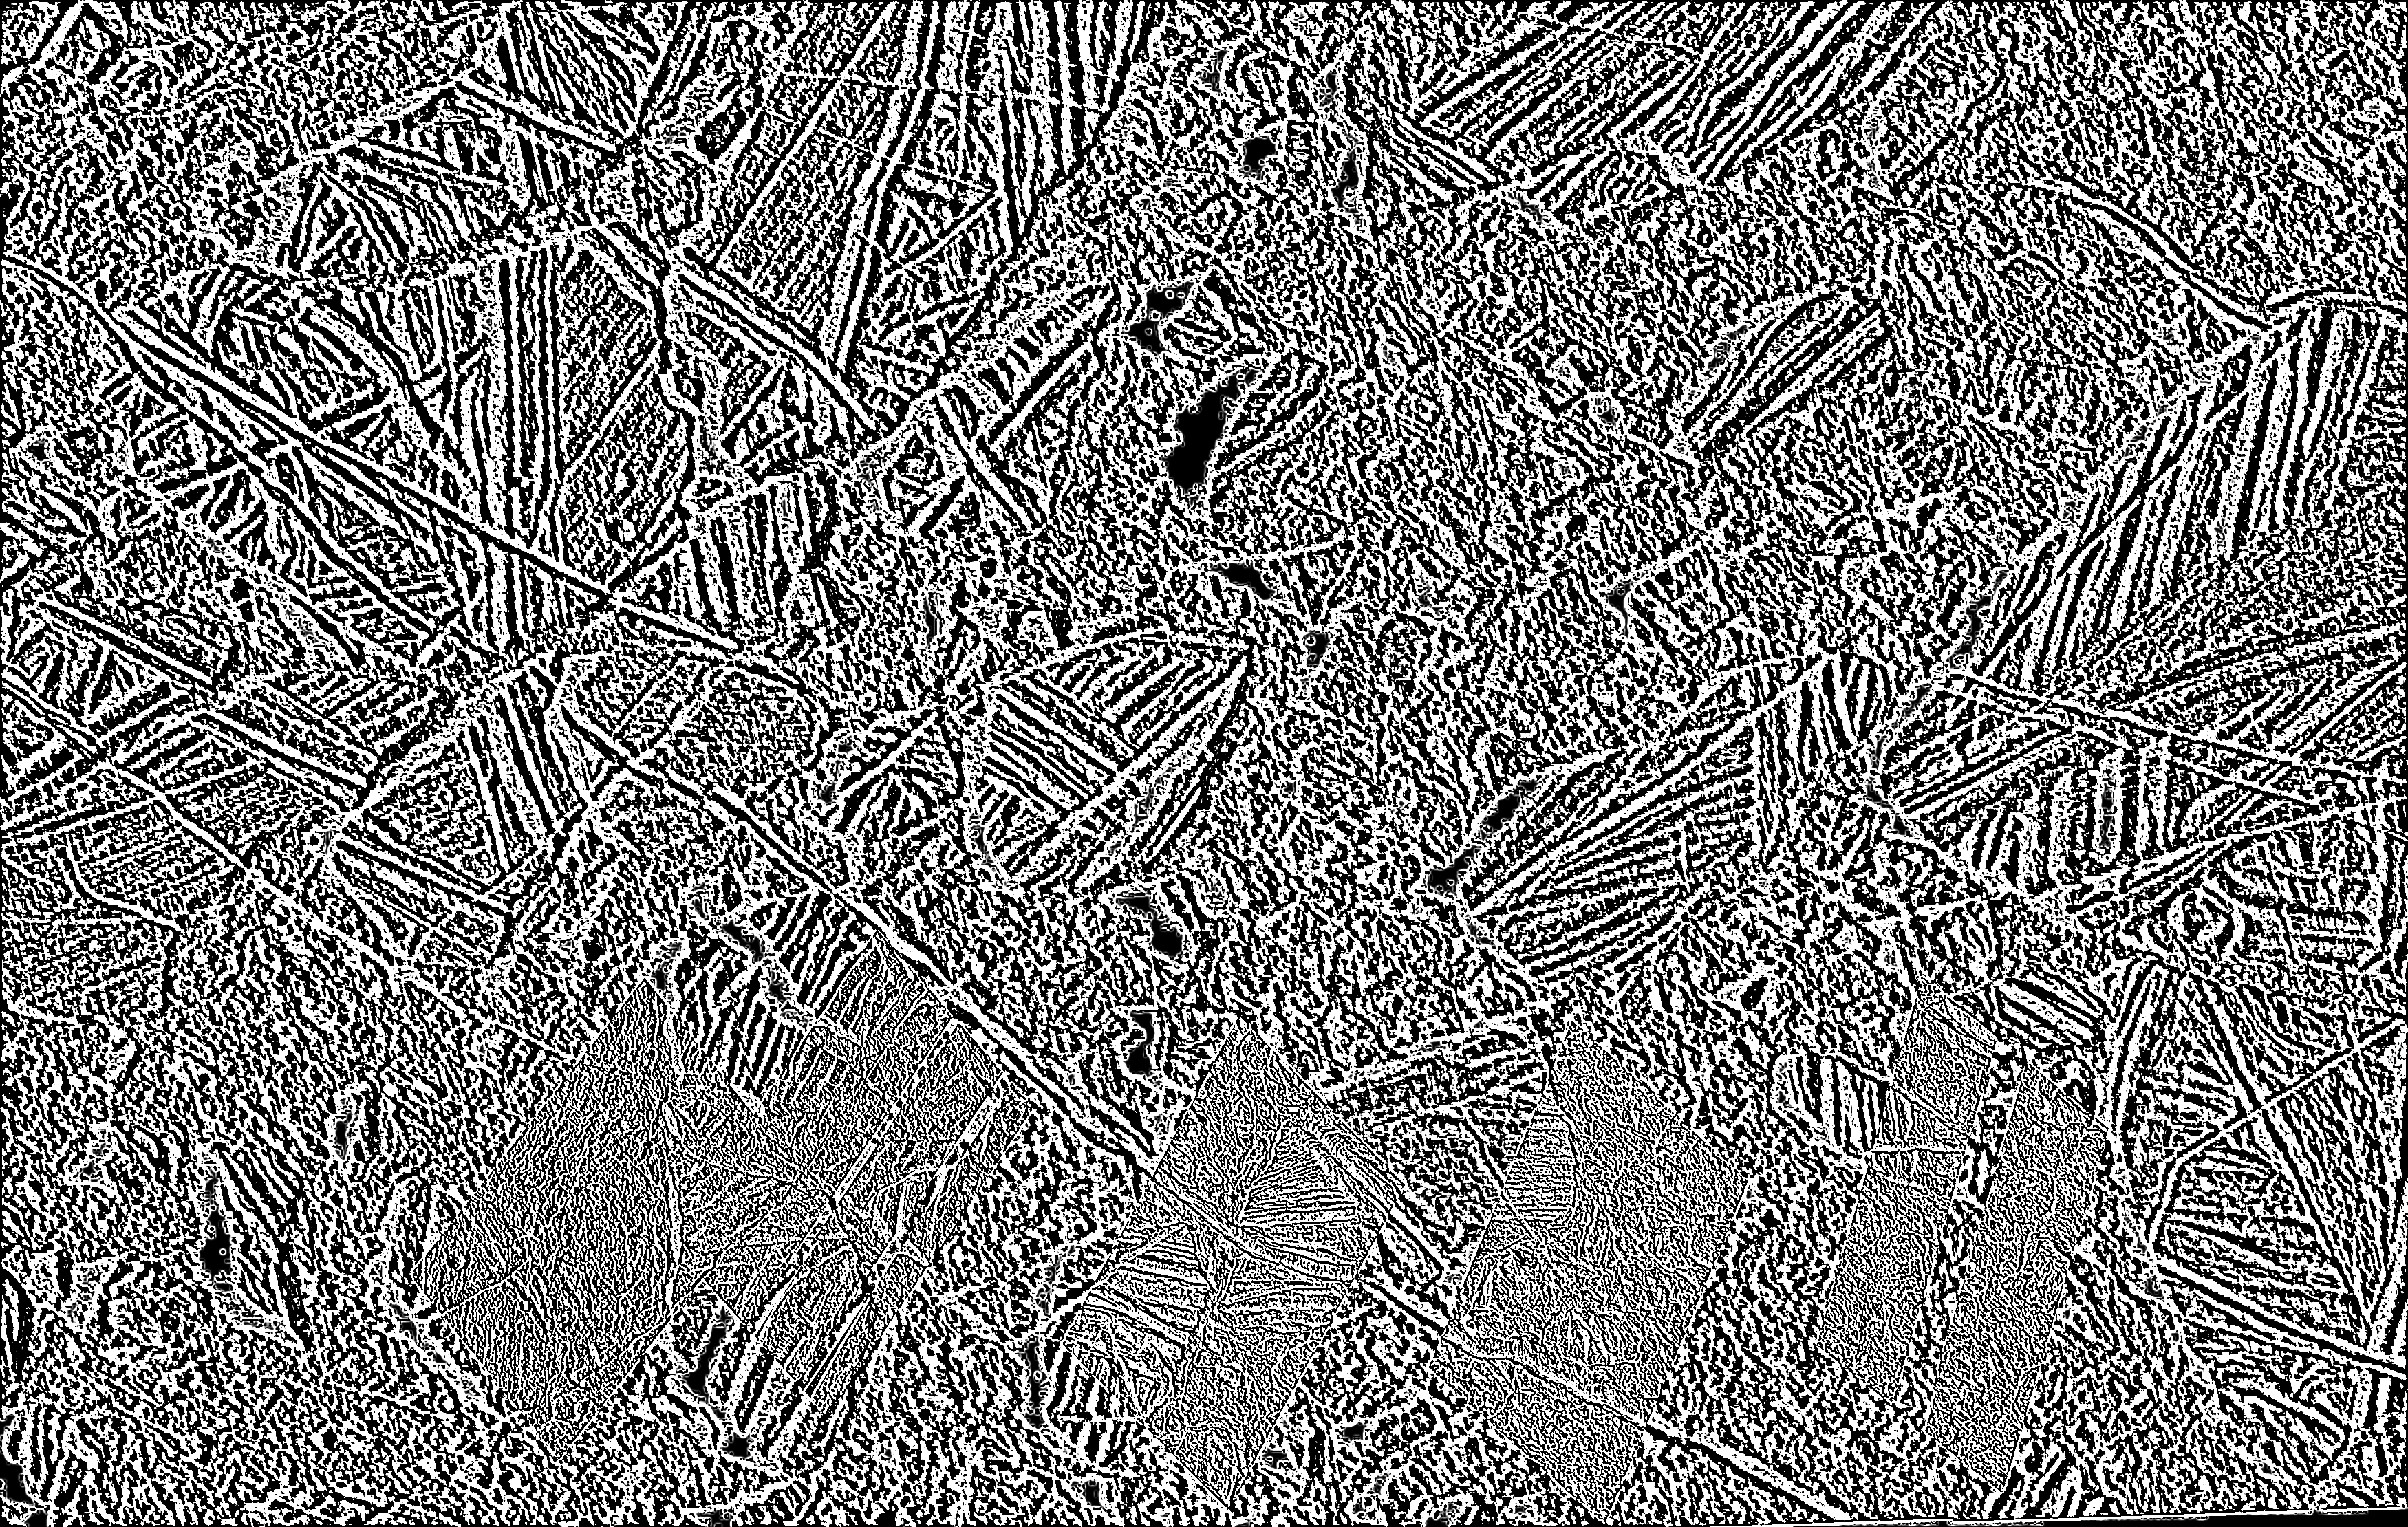
\includegraphics[width=.48\textwidth]{figures/edge/PIA01403_filtered}
	}
	\\
	\subfloat{
		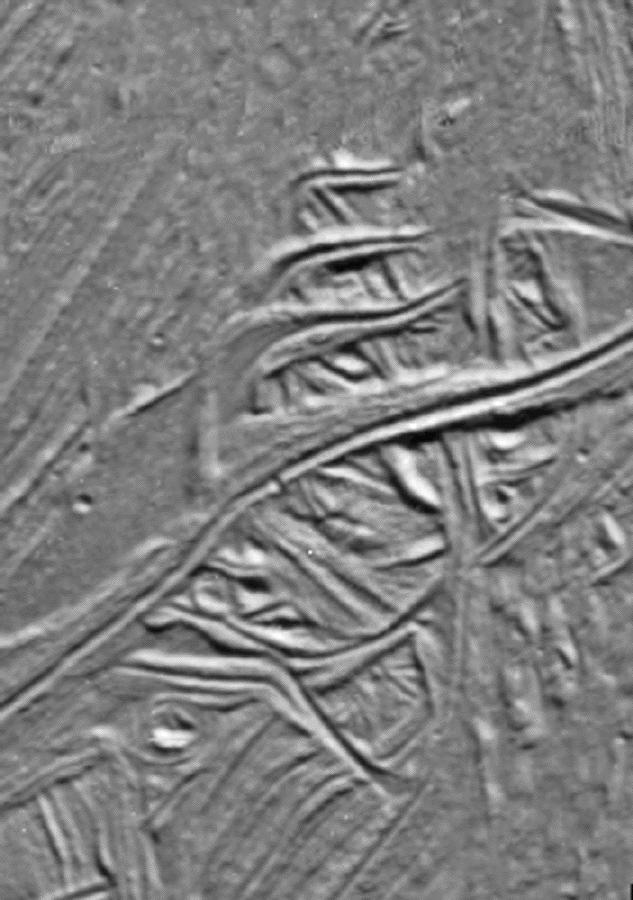
\includegraphics[width=.31\textwidth]{figures/edge/PIA01642}
	}
	\subfloat{
		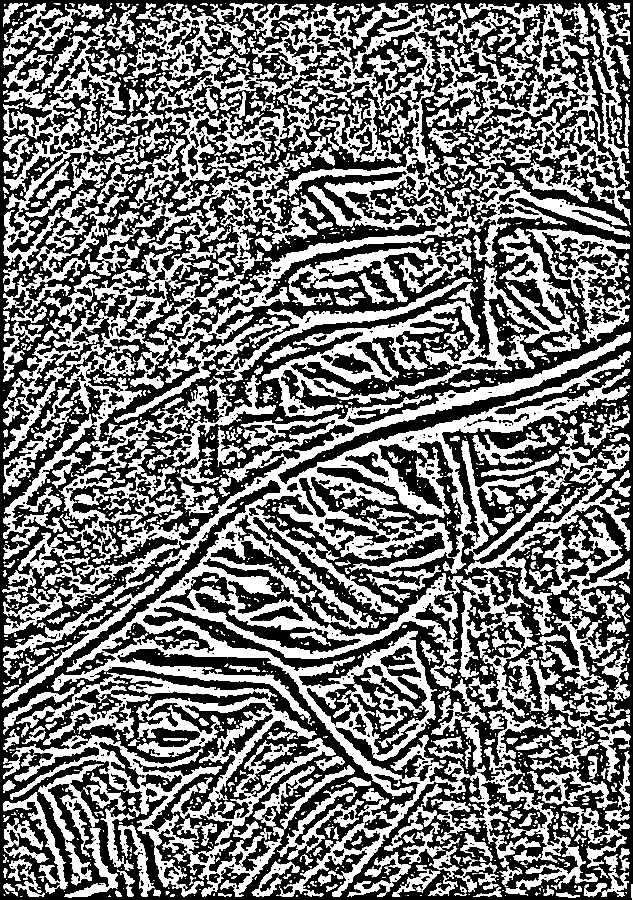
\includegraphics[width=.31\textwidth]{figures/edge/PIA01642_filtered}
	}
	\subfloat{
		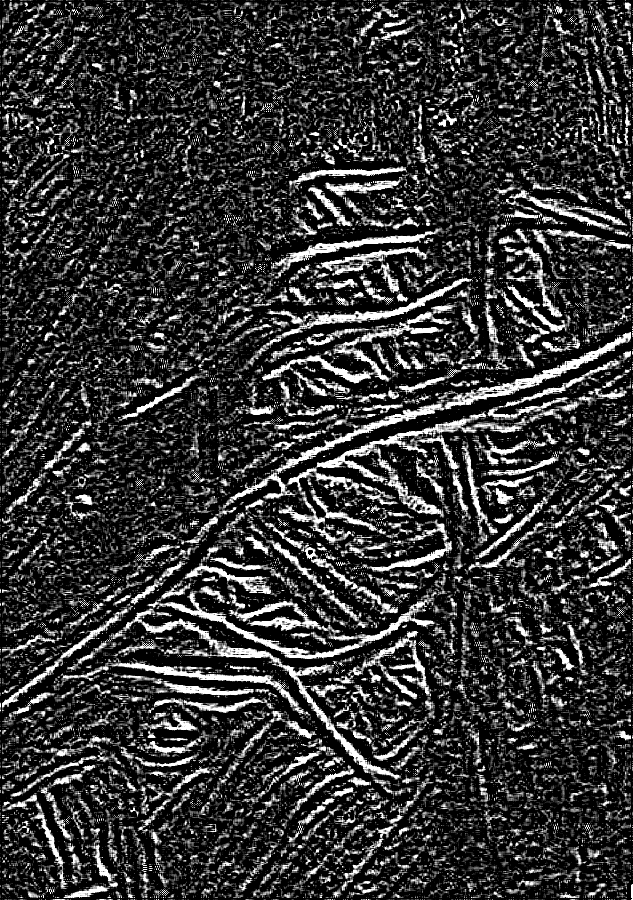
\includegraphics[width=.31\textwidth]{figures/edge/PIA01642_filtered_alternativ}
	}
	\captionsetup{width=.9\textwidth}
	\caption{Example of Laplacian Gaussian filter used for edge detection on the surface of the moon}
	\label{fig:edge_detection}
\end{figure}